\section{Approach}
\label{sec:approach}

Because of its superior popularity \TODO{prove}, in this work, we will confine ourselves to the JavaScript/npm ecosystem.
Our goal is thus to develop a tool for npm package developers that displays an overview of the downstream dependencies and their details for a chosen package.
Concretely, we pose the following key requirements to this tool:

\begin{enumerate}[label=R\arabic*]
	\item \label{req1} The tool allows package developers to survey and explore the usages of individual package members.
	\item The tool blends in well with the usual workflow of package developers.
	\item \label{req3} The tool runs out-of-the-box with a small footprint, without the user needing to perform any sophisticated setup steps or providing additional system resources for it to work.
\end{enumerate}

In essence, our proposed approach to fulfill these requirements consists of three steps:
\begin{enumerate*}
	\item collect downstream dependency repositories,
	\item mine package usage samples from them,
	and \item aggregate and present these usage data to the user.
\end{enumerate*}
In the following, we will describe each step.

\subsection{Downstream dependency collection}
\label{sec:approach/collection}

In the first step, a list of repositories that depend on the target package has to be assembled.
As mentioned in \cref{sec:related_work/usage_information}, many approaches start with a large downloaded corpus of unspecific repositories from the ecosystem which they then iterate over to filter the relevant repositories.
However, a major drawback of this approach is the high resource demand for both creating and traversing this corpus.
This approach is suited for analyzing repositories in large scale but is not conform to \cref{req1} due to the large footprint in terms of computational power and time.

As an alternative, we have decided to apply significantly stricter pre-filtering to the set of repositories before downloading it to the local machine.
For that, we have chosen two publicly available data sources:\footnote{
	Other data sources that we have rejected include GitHub code search which has limited precision results and is not freely accessible programatically as well as the \emph{libraries.io} service \citep{katz2020libraries} whose downstream dependency search was inoperative at the time of writing.%
}

\begin{enumerate}[label=(\roman*)]
	\item The npm registry which maintains a doubly-connected edge list of all npm packages that depend on each other.
	\item The code search engine \emph{Sourcegraph}\footnote{\url{https://sourcegraph.com/}} which is indexing repositories from most popular OSS platforms such as GitHub or GitLab.
		Using this search engine, we can query all repositories that declare a dependency on the target package in their package metadata file.
\end{enumerate}

Finally, we can download the source code for a small number of relevant repositories only.

\subsection{Usage sample mining}
\label{sec:approach/mining}

\begin{figure*}[htb!]
	\newcommand\lowlight[1]{\textcolor{gray}{#1}}
	\newcommand\highlight[1]{\textcolor{red}{#1}}
	\centering
	\begin{subfigure}[t]{.32\linewidth}
		\begin{tikzpicture}
	\node {CallExpression}
		child {node [accent1] {identifier}}
		child [gray] {node [gray, yshift = -0.5cm] {typeArguments}}
		child [gray] {node [gray] {arguments}};
\end{tikzpicture}
\caption[LoF entry]{
	Node pattern for a TypeScript functional call, such as in:

	\code{\textlowlight{result = }\uline{\texthighlight{fun}<\textlowlight{T1}, \textlowlight{T2}>(\textlowlight{arg1}, \textlowlight{arg2})}\textlowlight{;}}
}

	\end{subfigure}
	\hfill
	\begin{subfigure}[t]{.32\linewidth}
		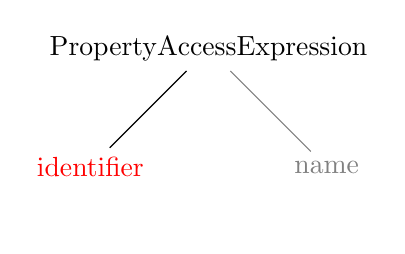
\begin{tikzpicture}
	\node {PropertyAccessExpression}
		child {node [red] {identifier}}
		child [white] {node [yshift = -0.5cm] {\phantom{node}}}  % ensure same height as sibling figures
		child [gray] {node [gray] {name}}
		;
\end{tikzpicture}
\caption[LoF entry]{
	Node pattern for a property access, such as in:

	\code{\lowlight{return }\uline{\lowlight{obj}.\highlight{prop}}\lowlight{;}}
}

	\end{subfigure}
	\hfill
	\begin{subfigure}[t]{.32\linewidth}
		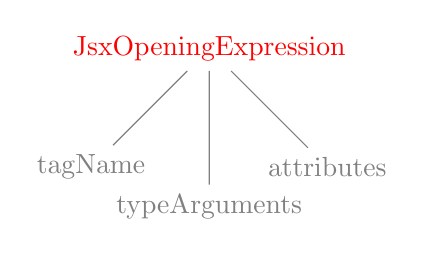
\begin{tikzpicture}
	\node [red] {JsxOpeningExpression}
		child [gray] {node [gray] {tagName}}
		child [gray] {node [gray, yshift = -0.5cm] {typeArguments}}
		child [gray] {node [gray] {attributes}};
\end{tikzpicture}
\caption[LoF entry]{
	Node pattern for a JSX opening tag, such as in:

	\code{\lowlight{elem = }\uline{<Button \lowlight{color}="\lowlight{blue}"> \lowlight{Google</Button>}}\lowlight{;}}
}

	\end{subfigure}

	\caption{AST patterns for example JavaScript/TypeScript expressions.
		The \highlight{highlighted} node contains the link to the declaration of the referenced identifier.
	}
	\label{fig:approach/mining/patterns}
\end{figure*}
\footnotetext{\url{https://reactjs.org/docs/introducing-jsx.html}}
\footnotetext{\url{https://www.typescriptlang.org/docs/handbook/jsx.html}}


Having downloaded the selected downstream dependency repositories, we can proceed to extract usage samples for the target package from each dependency repository.
Our goal is to identify these usage samples on a fine-granular level so that we can trace them down to the single identifiers that were exposed by the target package.

To do so, we start by parsing the source code of every dependency repository as well as the source of the target package each into a separate AST.

% TODO: use term "binding"?
In a second step, every dependency AST is traversed together with the target package AST in order to create links between semantically related nodes, e.g., between an expression and the variable it is assigned to, or between a function call and the definition of this function.

In the final step, we traverse the AST again and collect all nodes that are linked to a declaration in the target package.
To identify these links, we define a number of patterns for node structures and look up the declaration of every matched node (see \cref{fig:approach/mining/patterns}).

\subsection{Presentation of results}
\label{sec:approach/presentation}

After all references have been collected, a proper UI is still required to provide users easy access to these data that fulfills the requirements mentioned above.
To satisfy \cref{req2} and make our tool avaiable in the usual working environment of users, we implement it as an extension to a popular IDE.
One of the most popular IDEs that support JavaScript, and the one with the highest annual growth, is Visual Studio Code\footnote{\url{https://code.visualstudio.com/}}\footnote{Top IDE Index by Pierre Carbonnelle (2021): \url{https://pypl.github.io/IDE.html}}.
As it also provides a comprehensive set of APIs for extension developers, we have decided to roll our tool out as a VS Code extension.

For choosing appropriate views of the raw reference data, we have identified three common questions of package developers to answer each of which they require access to downstream dependencies and their usage samples:

\begin{enumerate}[label=Q\arabic*]
	\item Which dependencies do use the target package and what problems are they solving with it?
	\item By how many dependencies is a particular package member being used?
	\item In which contexts and constellations is a particular package member being used?
\end{enumerate}

To support developers in answering these questions and fulfill \cref{req1}, we have designed the following views for our extension:

\begin{enumerate}[label=(\roman*)]
	\item The \emph{dependency browser} allows to explore all downstream dependencies and, grouped for each dependency, all their references to the target package.
	\item The \emph{usage browser} displays all public package member and, grouped for each member, all dependencies and their references to this member.
	\item The \emph{CodeLens integration} provides quick access to a slice of the usage browser that is attached to the definition of each package member right in the source code editor.
\end{enumerate}

Both references and members are organized in a tree view reflecting the hierarchical structure of the original software repository.
In addition, we recognize the effort of browsing large lists of dependency data and encounter it by providing an ``I'm felling lucky'' button for every view that redirects the user to a random dependency resp. reference to gain a faster, unbiased impression of usage samples.
